\section{\color{red}Grafer}
En graf er en samling av kanter og noder. Vi kaller mengden av alle nodene $ V $ (verticies), og mengden av alle kantene $ E $ (edges). Grafen $ G $ blir da en samling av disse to mengdene. Formelt kan vi definere en graf slik:

\begin{definisjon}
En graf $ G $  er et par $ (V, E) $, der $ V $ er en ikke-tom mengde noder og $ E $ en mengde nodepar $ \{v_1, v_2\} $; $ v_1, v_2 \in V $ der $ \{v_1, v_2\} $ angir at grafen inneholder en kant fra $ v_1 $ til $ v_2 $.
\end{definisjon}

Vi bruker $ |E| $ for å betegne antall kanter og $ |V| $ for å betegne antall noder. 

Vi sier at en node er \textbf{nabo} med en annen node hvis de har en kant mellom seg. I figur \ref{fig:graf} er B og A naboer, men A og C er ikke naboer. 

En \textbf{sti} eller \textbf{vei} er en sekvens av noder (og kantene mellom dem) fra en node til en annen. En sti fra A til G i figuren under kan for eksempel være A, D, C, G. (siden grafen inneholder løkker er ikke stien entydig)

En graf er \textbf{rettet} hvis kantene har en spesiell retning, og \textbf{urettet} hvis vi ikke bryr oss om retningen på kantene. I en rettet graf vil kanten $ \{v_1, v_2\} $ bety at det går en kant fra $ v_1 $ til $ v_2 $, men ikke nødvendigvis fra $ v_2 $ til $ v_1 $. Grafen i figur \ref{fig:tre} er urettet. Hvis en graf er rettet kaller vi ofte naboene for \textbf{etterfølgere}. 

En graf er \textbf{vektet} hvis kantene har en verdi knyttet til seg, ofte kalt \emph{kosten} til kanten. I en \textbf{uvektet} graf har ikke kantene noen spesiell verdi. Vi kan tenke på en uvektet graf som en vektet graf der alle kantene har kost = 1.

Grafen er \textbf{syklisk} hvis den inneholder løkker, og \textbf{asyklisk} hvis den ikke inneholder løkker. I figur \ref{fig:graf} ser vi at A, B, C, D danner en løkke (det gjør også C, G, F, E). Grafen er derfor syklisk.

En type grafer vi jobber mye med er \textbf{DAG}er. DAG står for \emph{Directed Asyclic Graph}, på norsk: en rettet, asyklisk graf. 


\begin{figure}[H]
\centering
\caption{Eksempel på en urettet, uvektet graf}~\\
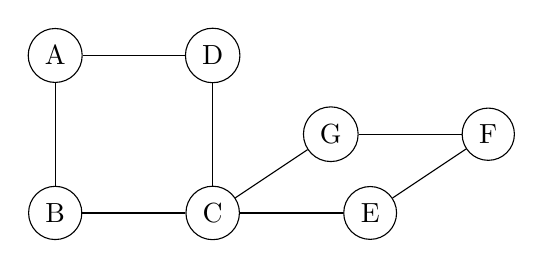
\begin{tikzpicture}
\tikzstyle{vertex} = [circle, draw=black]
\tikzstyle{edge} = [draw=black]

\node[vertex] (A) at (-1,0) {A};
\node[vertex] (B) at (-1,-2) {B};
\node[vertex] (C) at (1,-2) {C};
\node[vertex] (D) at (1,0) {D};
\node[vertex] (E) at (3,-2) {E};
\node[vertex] (F) at (4.5,-1) {F};
\node[vertex] (G) at (2.5, -1) {G};

\draw[edge] (B) -- (A);
\draw[edge] (B) -- (C);
\draw[edge] (A) -- (D);
\draw[edge] (C) -- (E);
\draw[edge] (C) -- (D);
\draw[edge] (E) -- (F);
\draw[edge] (C) -- (G);
\draw[edge] (G) -- (F);
\end{tikzpicture}
\label{fig:graf}
\end{figure}


\subsection{\color{red}Terminologi}

\subsubsection{Hamiltonsk sti}
En hamiltonsk sti er en sti som besøker alle nodene én gang. Dette kan virke som en triviell sak, men i en del tilfeller er det faktisk ikke mulig å finne en hamiltonsk sti. I grafen i figur \ref{fig:graf} er B, A, D, C, G, F, E en hamiltonsk sti (det finnes fler). 

Et berømt eksempel på en graf \emph{uten} en hamiltonsk sti er broene i Königsberg:
\begin{figure}[H]
\centering
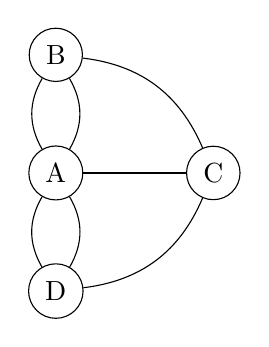
\begin{tikzpicture}
\tikzstyle{vertex} = [circle, draw=black]
\tikzstyle{edge} = [draw=black]

\node[vertex] (A) at (0,0) {A};
\node[vertex] (B) at (0,1.5) {B};
\node[vertex] (C) at (2,0) {C};
\node[vertex] (D) at (0, -1.5) {D};

\draw[edge] (A) to (C);
\draw[edge] (B) to [bend left] (C);
\draw[edge] (A) to [bend left] (B);
\draw[edge] (A) to [bend right] (B);
\draw[edge] (A) to [bend left] (D);
\draw[edge] (A) to [bend right] (D);
\draw[edge] (D) to [bend right] (C);
\end{tikzpicture}
\end{figure}



\subsubsection{Spenntrær}
Vi begynner med en definisjon:

\begin{definisjon}
Et \textbf{spenntre} for en urettet graf $ G $ er et tre med kanter fra grafen slik at alle nodene i $ G $ er forbundet. Spesielt er et \textbf{minimalt spenntre} de(t) spenntre(ene) med lavest total kostnad.
\end{definisjon}

\noindent Minimale spenntrær er sjeldent entydig bestemt. Vi har et entydig minimalt spenntre hvis alle kantene har forskjellig vekt. Vi tegner opp et eksempel:

\begin{figure}[H]
\centering
\caption{En graf (venstre) og et minimalt spenntre for grafen (høyre)}~\\
\label{fig:min_spenntre}
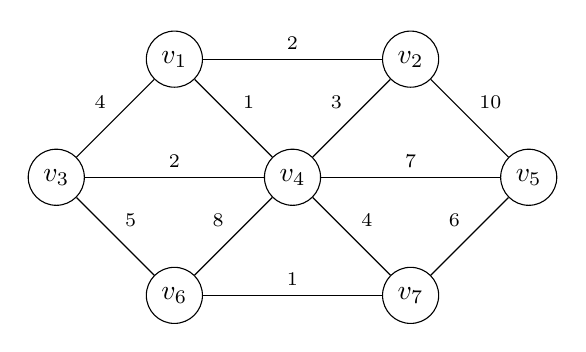
\begin{tikzpicture}[auto,node distance=2cm]
\tikzstyle{vertex} = [circle, draw=black]
\tikzstyle{edge} = [draw=black]

\node[vertex] (v1) at (-1.5,1.5) {$ v_1 $};
\node[vertex] (v2) at (1.5, 1.5) {$ v_2 $};
\node[vertex] (v3) at (-3,0) {$ v_3 $};
\node[vertex] (v4) at (0,0) {$ v_4 $};
\node[vertex] (v5) at (3,0) {$ v_5 $};
\node[vertex] (v6) at (-1.5,-1.5) {$ v_6 $};
\node[vertex] (v7) at (1.5,-1.5) {$ v_7 $};

\draw[edge] (v3) to node{\scriptsize4} (v1);
\draw[edge] (v3) to node{\scriptsize2} (v4);
\draw[edge] (v3) to node{\scriptsize5} (v6);
\draw[edge] (v1) to node{\scriptsize1} (v4);
\draw[edge] (v6) to node{\scriptsize8} (v4);
\draw[edge] (v4) to node{\scriptsize3} (v2);
\draw[edge] (v4) to node{\scriptsize4} (v7);
\draw[edge] (v4) to node{\scriptsize7} (v5);
\draw[edge] (v2) to node{\scriptsize10} (v5);
\draw[edge] (v7) to node{\scriptsize6} (v5);
\draw[edge] (v1) to node{\scriptsize2} (v2);
\draw[edge] (v6) to node{\scriptsize1} (v7);
\end{tikzpicture}~~
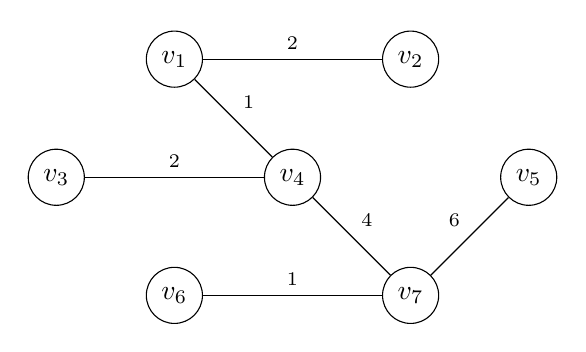
\begin{tikzpicture}[auto,node distance=2cm]
\tikzstyle{vertex} = [circle, draw=black]
\tikzstyle{edge} = [draw=black]

\node[vertex] (v1) at (-1.5,1.5) {$ v_1 $};
\node[vertex] (v2) at (1.5, 1.5) {$ v_2 $};
\node[vertex] (v3) at (-3,0) {$ v_3 $};
\node[vertex] (v4) at (0,0) {$ v_4 $};
\node[vertex] (v5) at (3,0) {$ v_5 $};
\node[vertex] (v6) at (-1.5,-1.5) {$ v_6 $};
\node[vertex] (v7) at (1.5,-1.5) {$ v_7 $};

\draw[edge] (v3) to node{\scriptsize2} (v4);
\draw[edge] (v1) to node{\scriptsize1} (v4);
\draw[edge] (v4) to node{\scriptsize4} (v7);
\draw[edge] (v7) to node{\scriptsize6} (v5);
\draw[edge] (v1) to node{\scriptsize2} (v2);
\draw[edge] (v6) to node{\scriptsize1} (v7);
\end{tikzpicture}~\\~\\
\end{figure}

For å finne et minimalt spenntre til en graf kan vi bruke Prims algoritme (\ref{prim}) eller Kruskals algoritme (\ref{kruskal})


\subsubsection{Topologisk sortering}
Topologisk sortering er en ordning av noder i en DAG slik at dersom det finnes en vei fra $ v_i $ til $ v_j $ i grafen kommer $ v_i $ før $ v_j $ i sorteringa. En topologisk sortering er ikke nødvendigvis entydig bestemt, ofte finnes det veldig mange. Hvis en graf er syklisk eksisterer det ikke en topologisk sortering av grafen. Vi ser på et eksempel: 

\begin{eks} Gitt følgende graf, finn alle topologiske sorteringer.
\begin{figure}[H]
\centering
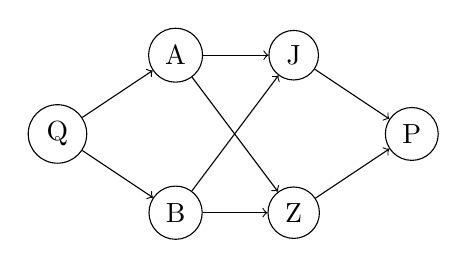
\begin{tikzpicture}[->]
\tikzstyle{v} = [circle, draw=black]
\tikzstyle{e} = [draw=black]

\node[v] (Q) at (-3, 0) {Q};
\node[v] (A) at (-1.5, 1) {A};
\node[v] (B) at (-1.5, -1) {B};
\node[v] (J) at (0, 1) {J};
\node[v] (Z) at (0, -1) {Z};
\node[v] (P) at (1.5, 0) {P};

\draw[e] (Q) to (A);
\draw[e] (Q) to (B);
\draw[e] (A) to (J);
\draw[e] (B) to (Z);
\draw[e] (B) to (J);
\draw[e] (A) to (Z);
\draw[e] (J) to (P);
\draw[e] (Z) to (P);
\end{tikzpicture}
\end{figure}

Vi ser at Q har inngrad 0, det er derfor et logisk sted å begynne. Etter Q kommer A og B. Vi ser at vi kan ikke gå videre fra A før uten å ha vært innom B, siden både J og Z er avhengige av B. Tilsvarende kan vi ikke gå videre fra B før vi har vært innom A. Til slutt ser vi at P er avhengig av både J og Z. Begge de to må derfor komme før P i sorteringa. Vi har da dekt alle mulige utfall. Vi kan liste opp alle mulige sorteringer:
\begin{itemize}
\item Q, A, B, J, Z, P
\item Q, B, A, J, Z, P
\item Q, A, B, Z, J, P
\item Q, B, A, Z, J, P
\end{itemize}

Vi kan ta med et moteksempel også: Q, A, J, B, Z, P er ikke en gyldig topologisk sortering siden J kommer før B i sorteringa, men i grafen ser vi at J er avhengig av B (det går en kant fra B til J).
\end{eks}



\subsubsection{Strongly connected components (SCC)}
Vi ser på definisjonen av strongly connected components (heretter SCC):
\begin{definisjon}
Anta at vi har en rettet graf $ G = (V, E) $. Vi har da at en \textbf{SCC} av $ G $ er et maksimalt sett av noder $ U \subseteq V $ slik at for alle $ u_1 $, $ u_{2} \in U $ har vi at $ u_1 \leadsto u_2 $ og $ u_2 \leadsto u_1 $.
\end{definisjon}

Med andre ord: en SCC er en del (partisjon) av grafen der alle nodene i den partisjonen kan nå alle andre noder i partisjonen. Vi ser på et eksempel:

\begin{eks} Finn alle SCCer i grafen:
\begin{figure}[H]
\centering
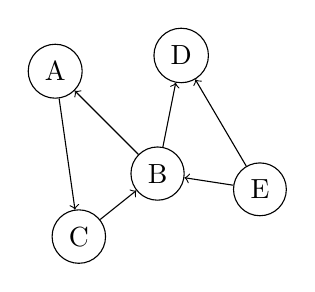
\begin{tikzpicture}[->]
\tikzstyle{v} = [circle, draw=black]
\tikzstyle{e} = [draw=black]

\node[v] (A) at (-1.3, 1.3) {A};
\node[v] (B) at (0, 0) {B};
\node[v] (C) at (-1, -.8) {C};
\node[v] (D) at (0.3, 1.5) {D};
\node[v] (E) at (1.3, -0.2) {E};

\draw[e] (A) to (C);
\draw[e] (C) to (B);
\draw[e] (B) to (A);
\draw[e] (B) to (D);
\draw[e] (E) to (B);
\draw[e] (E) to (D);
\end{tikzpicture}
\end{figure}
Vi ser at \{A, B, C\} danner en SCC. D har ingen kanter ut. Den må derfor være sin egen SCC. E ingen kanter inn, den må også være sin egen SCC. Vi har da at vi kan partisjonere grafen slik: \{\{A, B, C\}, \{D\}, \{E\} \}
\end{eks}

\subsubsection{\color{red}Articulation points og biconnectivity}


\subsection{\color{red}Grafalgoritmer}

\subsubsection{\color{red}Dybde først}


\subsubsection{\color{red}Finne SCC}

\subsubsection{\color{red}Dijkstras algoritme}
\label{dijkstra}

\subsubsection{\color{red}Prims algoritme}
\label{prim}

\subsubsection{\color{red}Kruskals algoritme}
\label{kruskal}

\subsubsection{\color{red}Floyds algoritme}
\label{floyd}